%Version 2.1 April 2023
% See section 11 of the User Manual for version history
%
%%%%%%%%%%%%%%%%%%%%%%%%%%%%%%%%%%%%%%%%%%%%%%%%%%%%%%%%%%%%%%%%%%%%%%
%%                                                                 %%
%% Please do not use \input{...} to include other tex files.       %%
%% Submit your LaTeX manuscript as one .tex document.              %%
%%                                                                 %%
%% All additional figures and files should be attached             %%
%% separately and not embedded in the \TeX\ document itself.       %%
%%                                                                 %%
%%%%%%%%%%%%%%%%%%%%%%%%%%%%%%%%%%%%%%%%%%%%%%%%%%%%%%%%%%%%%%%%%%%%%

%%\documentclass[referee,sn-basic]{sn-jnl}% referee option is meant for double line spacing

%%=======================================================%%
%% to print line numbers in the margin use lineno option %%

%%\documentclass[lineno,sn-basic]{sn-jnl}% Basic Springer Nature Reference Style/Chemistry Reference Style

%%======================================================%%
%% to compile with pdflatex/xelatex use pdflatex option %%
%%======================================================%%

%%\documentclass[pdflatex,sn-basic]{sn-jnl}% Basic Springer Nature Reference Style/Chemistry Reference Style


%%Note: the following reference styles support Namedate and Numbered referencing. By default the style follows the most common style. To switch between the options you can add or remove “Numbered” in the optional parenthesis.
%%The option is available for: sn-basic.bst, sn-vancouver.bst, sn-chicago.bst, sn-mathphys.bst. %

%%\documentclass[sn-nature]{sn-jnl}% Style for submissions to Nature Portfolio journals
%%\documentclass[sn-basic]{sn-jnl}% Basic Springer Nature Reference Style/Chemistry Reference Style
\documentclass[pdflatex,sn-mathphys,Numbered]{sn-jnl}% Math and Physical Sciences Reference Style
%%\documentclass[sn-aps]{sn-jnl}% American Physical Society (APS) Reference Style
%%\documentclass[sn-vancouver,Numbered]{sn-jnl}% Vancouver Reference Style
%%\documentclass[sn-apa]{sn-jnl}% APA Reference Style
%%\documentclass[sn-chicago]{sn-jnl}% Chicago-based Humanities Reference Style
%%\documentclass[default]{sn-jnl}% Default
%%\documentclass[default,iicol]{sn-jnl}% Default with double column layout

%%%% Standard Packages
%%<additional latex packages if required can be included here>

\usepackage{graphicx}%
\usepackage{multirow}%
\usepackage{amsmath,amssymb,amsfonts}%
\usepackage{amsthm}%
\usepackage{mathrsfs}%
\usepackage[title]{appendix}%
\usepackage{xcolor}%
\usepackage{textcomp}%
\usepackage{manyfoot}%
\usepackage{booktabs}%
\usepackage{algorithm}%
\usepackage{float}%
\usepackage{algorithmicx}%
\usepackage{algpseudocode}%
\usepackage{listings}%
\usepackage{graphicx}
\usepackage{threeparttable}
\usepackage{tablefootnote}
\usepackage{url}
% \usepackage{breakurl}
\usepackage{xurl}
\hypersetup{hypertexnames=false}


%%%%

%%%%%=============================================================================%%%%
%%%%  Remarks: This template is provided to aid authors with the preparation
%%%%  of original research articles intended for submission to journals published
%%%%  by Springer Nature. The guidance has been prepared in partnership with
%%%%  production teams to conform to Springer Nature technical requirements.
%%%%  Editorial and presentation requirements differ among journal portfolios and
%%%%  research disciplines. You may find sections in this template are irrelevant
%%%%  to your work and are empowered to omit any such section if allowed by the
%%%%  journal you intend to submit to. The submission guidelines and policies
%%%%  of the journal take precedence. A detailed User Manual is available in the
%%%%  template package for technical guidance.
%%%%%=============================================================================%%%%

%\jyear{2021}%

%% as per the requirement new theorem styles can be included as shown below
%% The theorem-like environments from the template are not used in this manuscript.
%%\theoremstyle{thmstyleone}%
%%\newtheorem{theorem}{Theorem}%  meant for continuous numbers
%%\newtheorem{theorem}{Theorem}[section]% meant for sectionwise numbers
%% optional argument [theorem] produces theorem numbering sequence instead of independent numbers for Proposition
%%\newtheorem{proposition}[theorem]{Proposition}%
%%\newtheorem{proposition}{Proposition}% to get separate numbers for theorem and proposition etc.

%%\theoremstyle{thmstyletwo}%
%%\newtheorem{example}{Example}%
%%\newtheorem{remark}{Remark}%

%%\theoremstyle{thmstylethree}%
%%\newtheorem{definition}{Definition}%

\raggedbottom
%%\unnumbered% uncomment this for unnumbered level heads

\begin{document}

\title[Article Title]{Cross-border offshore hydrogen trade and carbon mitigation in Europe}

% Offshore Green Hydrogen Exports from Island Nations: Reshaping Europe’s Net-Zero Pathway

% Cross-border trading flows and carbon mitigation potential of offshore green hydrogen for Europe's net zero transition

%%=============================================================%%
%% Prefix	-> \pfx{Dr}
%% GivenName	-> \fnm{Joergen W.}
%% Particle	-> \spfx{van der} -> surname prefix
%% FamilyName	-> \sur{Ploeg}
%% Suffix	-> \sfx{IV}
%% NatureName	-> \tanm{Poet Laureate} -> Title after name
%% Degrees	-> \dgr{MSc, PhD}
%% \author*[1,2]{\pfx{Dr} \fnm{Joergen W.} \spfx{van der} \sur{Ploeg} \sfx{IV} \tanm{Poet Laureate}
%%                 \dgr{MSc, PhD}}\email{iauthor@gmail.com}
%%=============================================================%%

\author[1,2]{\fnm{Sheng} \sur{Wang}}\email{sheng.wang@newcastle.ac.uk}

\author[2,3]{\fnm{Muhammad} \sur{Maladoh Bah}}\email{muhammad.maladohbah@seai.ie}

% \author[4]{\fnm{Zeyuan} \sur{Xu}}\email{}


\affil*[1]{\orgdiv{School of Engineering}, \orgname{Newcastle University}, \orgaddress{\street{Newcastle University}, \city{Newcastle upon Tyne}, \postcode{NE17RU}, \country{The United Kingdom}}}

\affil[2]{\orgdiv{School of Electrical and Electronic Engineering}, \orgname{University College Dublin}, \orgaddress{\street{Belfield}, \city{Dublin}, \postcode{D04 V1W8}, \country{Ireland}}}

\affil[3]{ \orgname{Sustainable Energy Authority Of Ireland}, \orgaddress{\street{3 Park Place, Hatch Street}, \city{Dublin}, \postcode{D02 FX65}, \country{Ireland}}}

% \affil[4]{\orgdiv{Department of Chemical and Biomolecular Engineering}, \orgname{National University of Singapore}, \orgaddress{\city{Singapore}, \postcode{117585}, \country{Singapore}}}

%%==================================%%
%% sample for unstructured abstract %%
%%==================================%%

\abstract{
European countries are pursuing the net-zero transition and offshore energy-resource development. Ireland and the UK have announced 2050 offshore wind ambitions of 37 and 125 GW, more than twice projected domestic power demand, while continental demand centres such as Germany are calling for cleaner fuel resources. Exporting surplus offshore green hydrogen could bridge this supply-demand imbalance and mitigate emissions across Europe. Yet the roles of these island countries are often underestimated when offshore hydrogen is assessed mainly by production cost. Here we develop an integrated European assessment linking cost-supply curves, hourly power-gas operation, hydrogen/ammonia shipping, national demand and external import competition from 2030 to 2050. Results indicate that the UK will be the largest hydrogen supplier from 2030 to 2050, while Ireland nearly matches it in 2050, with both reaching about 162 TWh yr$^{-1}$ of net exports. This export potential could reduce 175.5 Mt CO$_2$ yr$^{-1}$ of carbon dioxide emissions in Europe in 2050. This general flow of hydrogen from the west to the east not only facilitates Europe's net-zero progress, but also reshapes the energy supply structure and helps to ensure energy security across the European continent.
}

%%================================%%
%% Sample for structured abstract %%
%%================================%%

% \abstract{\textbf{Purpose:} The abstract serves both as a general introduction to the topic and as a brief, non-technical summary of the main results and their implications. The abstract must not include subheadings (unless expressly permitted in the journal's Instructions to Authors), equations or citations. As a guide the abstract should not exceed 200 words. Most journals do not set a hard limit however authors are advised to check the author instructions for the journal they are submitting to.
%
% \textbf{Methods:} The abstract serves both as a general introduction to the topic and as a brief, non-technical summary of the main results and their implications. The abstract must not include subheadings (unless expressly permitted in the journal's Instructions to Authors), equations or citations. As a guide the abstract should not exceed 200 words. Most journals do not set a hard limit however authors are advised to check the author instructions for the journal they are submitting to.
%
% \textbf{Results:} The abstract serves both as a general introduction to the topic and as a brief, non-technical summary of the main results and their implications. The abstract must not include subheadings (unless expressly permitted in the journal's Instructions to Authors), equations or citations. As a guide the abstract should not exceed 200 words. Most journals do not set a hard limit however authors are advised to check the author instructions for the journal they are submitting to.
%
% \textbf{Conclusion:} The abstract serves both as a general introduction to the topic and as a brief, non-technical summary of the main results and their implications. The abstract must not include subheadings (unless expressly permitted in the journal's Instructions to Authors), equations or citations. As a guide the abstract should not exceed 200 words. Most journals do not set a hard limit however authors are advised to check the author instructions for the journal they are submitting to.}

\keywords{hydrogen, offshore wind, carbon mitigation, international trade}

%%\pacs[JEL Classification]{D8, H51}

%%\pacs[MSC Classification]{35A01, 65L10, 65L12, 65L20, 65L70}

\maketitle

\section{Introduction}\label{sec1}

Offshore wind offers a promising solution for achieving net-zero ambitions in Europe,
especially for island countries. For example, Ireland and the UK have announced
offshore wind development plans reaching 37 and 125 GW of installed capacity,
respectively, by 2050 \cite{FutureFrameworkfor, Offshorewindnetzero}. These targets
are highly ambitious because they are more than twice the projected values of their
overall power demands in 2050 \cite{TenYearGenerationCapacity, FES}. At this scale,
local power systems cannot fully utilise the resulting offshore wind volumes, leaving
surplus generation that increases connection bottlenecks, curtailment risk and
real-time balancing pressures.

These countries' significant offshore wind ambitions therefore create an important
role for green hydrogen. Produced from renewable electricity through electrolysis,
green hydrogen avoids the direct operational emissions associated with fossil-based
hydrogen routes \cite{Comparisonoftheemissions}. As a storable and transportable
energy carrier, hydrogen can absorb offshore wind that cannot be fully accommodated
by domestic power systems, reduce curtailment pressure, and move renewable energy
across time, sectors and borders. It can be used in domestic industry, heat, power
and gas systems, or transported through shipping and gas networks to distant demand
centres. This export pathway is important because surplus offshore wind in Ireland
and the UK coincides with growing hydrogen demand in continental Europe. Germany
expects annual imported hydrogen needs of 45--77 TWh by 2030
\cite{TheNationalHydrogenStrategy, HydrogenWhichimport}, and Belgium has identified
20 TWh of imported hydrogen demand by 2030 \cite{BelgianfederalHydrogenStrategy}.
Linking exporting and importing countries can ease offshore wind absorption pressures
in Ireland and the UK while supplying low-carbon fuels to hard-to-decarbonise sectors
across continental Europe.

Cost remains a central factor shaping the large-scale production and utilisation
of offshore green hydrogen, and it will strongly influence the development of
future international hydrogen trade. The levelised cost of hydrogen (LCOH) in
2030 is projected to be around 54--184 €/MWh, a range that overlaps with blue
hydrogen with carbon capture and storage (CCS) and green hydrogen from onshore
wind \cite{GlobalHydrogenReview2023}. In Ireland, offshore wind capacity is
expected to exceed onshore wind capacity around 2035 because of richer wind
resources, higher capacity factors and fewer land-use restrictions
\cite{windenergyroadmap}. Previous studies have evaluated offshore hydrogen
costs in individual European countries and regions, including North Sea countries
\cite{rogeau2023techno}, the UK \cite{giampieri2024techno}, Poland
\cite{komorowska2023evaluating}, and the Iberian Peninsula
\cite{gonzalez2024techno, calado2024assessment}. These studies provide LCOH
projections to 2050, with detailed cost breakdowns, production and transmission
routes, and uncertainty analyses. However, few studies compare the cost
competitiveness of different countries within a unified framework, which is
needed to understand how offshore hydrogen costs may shape the future European
hydrogen trading landscape.

European policy documents have identified several major hydrogen import routes,
including supplies from North Sea countries (Denmark, Germany and the Netherlands),
North Africa, the Middle East and the Americas. By contrast, the export potential
of Ireland and the UK, despite their Atlantic offshore wind resources, remains
less quantified. Recent Irish and UK policy and consulting reports have recognised
green-hydrogen export opportunities \cite{HydrogenImport, FutureFrameworkfor}, but
they provide limited quantitative evidence on offshore hydrogen costs, export
potential and transport choices. In particular, Irish export assessments have often
focused on a pipeline connection to France, leaving shipping-based hydrogen and
ammonia trade underexplored. More broadly, single-country studies cannot determine
how European hydrogen imports and exports should be allocated across countries.
An integrated analysis is therefore needed to assess how offshore hydrogen trade
can allocate renewable resources, contribute to Europe-wide decarbonisation, and
inform investment and infrastructure planning.

In this work, we for the first time investigate the roles of offshore hydrogen, especially the export from Ireland and the UK, in the decarbonization of the entire Europe.
First, we developed a unified bottom-up framework to assess the potential and cost-competitiveness of offshore hydrogen produced by major coastal countries in Europe. High spatial-temporal resolution geo-based meteorological data and social-economic data across Europe are used to simulate the wake effect and quantity-cost supply curves of offshore hydrogen for each country.
Secondly, using Ireland as an example, we proposed a new coordinated optimisation framework for power and gas systems to evaluate the domestic integration and export potentials of offshore electricity and hydrogen. The power and gas systems are coupled by gas-fired power plants and electrolysers, where bidirectional energy exchange is allowed to further activate the flexibility of whole energy systems. Various hydrogen integration schemes (including hydrogen blending and pure hydrogen), corresponding physical constraints, and the evolution of power system operating codes (such as inertia, must-run units, and system non-synchronous generation (SNSP)) are modelled in future scenarios.
Based on the cost-supply curves and exporting potential derived above, we then formulate an optimal international trading model to project the hydrogen flows among countries in 2030, 2040, and 2050. We further use a lowest-LCOH allocation as a counterfactual benchmark and vary external import prices to ensure the robustness of the resulting trade pattern. Then, the overall landscape of offshore hydrogen in Europe's net-zero transition, as well as the contributions from each country, becomes clear. These key findings can further strengthen confidence in the continuous investment in offshore facilities and help the governments with more bespoke offshore policy design.


\section{Results}

\subsection{Cost-competitiveness of green hydrogen production in coastal European countries}

We first consider eleven coastal European countries within the assessment scope: Belgium, Denmark, France, Germany, Ireland, the Netherlands, Norway, Portugal, Spain, Sweden, and the United Kingdom (UK). The selection captures countries with large exclusive economic zones (EEZs) for offshore infrastructure development and the principal coastal nodes connected through relatively direct European sea routes. Historical meteorological data for offshore wind-resource modelling, including wind speed, air pressure, and temperature, are obtained from the ERA-5 product at 1 h and 0.5$^\circ$ $\times$ 0.5$^\circ$ temporal and spatial resolutions \cite{ERA5}. Hourly capacity factors and wake-effect losses are simulated using the power curve and deployment assumptions of a 15 MW offshore wind turbine \cite{musial2019oregon}; the turbine power curve and wake-effect setup are shown in Supplementary Figs. 2--4. The resulting wind-speed probability distributions across national EEZs are presented in Fig. \ref{fig LCOH map}b. Ireland has the richest wind resource, with the highest modal wind speed, followed by the UK, largely because both countries are exposed to Atlantic wind conditions. Compared with continental countries, these two island countries show higher probabilities of strong wind speeds and a more even distribution of wind resources across the year.

Using these capacity factors and the assumed development, capital, operating and decommissioning costs of the offshore hydrogen production platform (including wind turbines, foundations and electrolysers; see Supplementary Figs. 5--10 and Supplementary Tables 3 and 4), we estimate the spatial LCOH distribution shown in Fig. \ref{fig LCOH map}a. The model also accounts for bathymetry, port locations, and connection points to the power and gas networks, allowing water depth, maintenance distance and network-connection distance to influence site-level costs \cite{bathymetry_2022, EMODnet}. The estimated LCOH ranges from 84.93 to more than 200 €/MWh across the studied EEZs. Denmark has the lowest LCOH, supported by high capacity factors and a shallow continental shelf. This lower bound approaches the blue-hydrogen benchmark, although it remains 33.94 \% higher than the onshore blue-hydrogen value of 68.92 €/MWh \cite{Globalaveragelevelised}. The UK's LCOH ranges from 85.97 to 307.26 €/MWh, giving it the second-lowest lower-bound LCOH. Ireland's LCOH ranges from 90.42 to 201.8 €/MWh, making it less cost-competitive than the leading countries despite its strong wind resource.

\begin{figure}
    \centering
    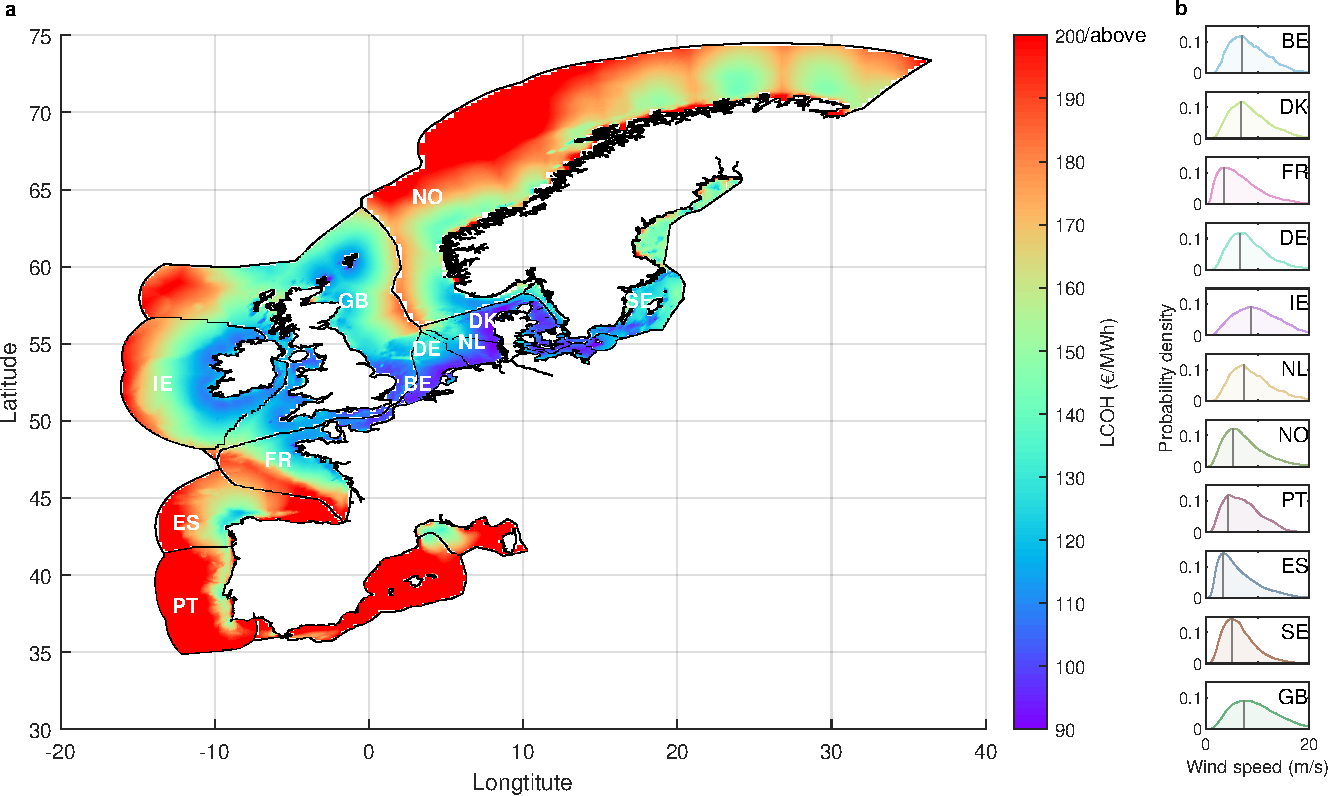
\includegraphics[width = 0.99\columnwidth]{figs/fig_LCOH_map_manu.pdf}
    \caption{\textbf{LCOH map and wind speed in coastal European countries.} \textbf{a} LCOH map in EEZs of coastal European countries. The black line outlines the EEZs. \textbf{b} Probability density of wind speed for each country. The vertical grey line in each figure shows the wind speed most likely to occur. BE, DK, FR, DE, IE, NL, NO, PT, ES, SE, and GB are the abbreviations for Belgium, Denmark, France, Germany, Ireland, The Netherlands, Norway, Portugal, Spain, Sweden, and the United Kingdom, respectively.}
    \label{fig LCOH map}
\end{figure}

After accounting for wake losses, vessel density, excluded areas (such as military and aquaculture areas), and future technology cost reductions \cite{wiser2021expert}, we derive hydrogen cost-supply curves for 2030, 2040 and 2050 (Fig. \ref{fig LCOH curve}). These constraints affect the effective power density available for offshore wind deployment; the supporting vessel-density, power-density and cost-reduction inputs are shown in Supplementary Figs. 11 and 12.
In 2030, the marginal LCOHs of Ireland and the UK are 76.10 and 79.02 €/MWh, respectively (Fig. \ref{fig lcoh rank}), with Ireland slightly lower than the UK. At equal production volumes, however, Ireland's LCOH is generally higher than the UK's. At low production volumes, Ireland is more cost-competitive than Portugal, Spain, Norway and Sweden, but it becomes less competitive than Sweden once capacity exceeds 10 GW. Within the first 5 GW, the UK remains close to Denmark's cost level, supporting an early cost advantage for offshore hydrogen production. Beyond this range, the UK still retains lower costs than most other countries. However, because the UK's offshore wind target is more ambitious, its marginal LCOH ranks eighth. This means that countries with lower marginal LCOHs, such as France and the Netherlands, can still supply limited volumes of competitive hydrogen despite having higher overall cost-supply curves. At this stage, offshore green hydrogen remains above the blue-hydrogen benchmark in most countries.

By 2040, technology and supply-chain learning reduce LCOH by around 21\% \cite{wiser2021expert}. As offshore wind capacity targets expand, country cost rankings also shift. Ireland's marginal LCOH reaches 67.40 €/MWh and becomes higher than those of the UK, Sweden and France, because its larger offshore capacity target pushes production into higher-cost sites. The UK moves ahead of Sweden in the ranking because of its favourable offshore conditions, including capacity factors, water depth and coastline length. Denmark remains the leading cost-competitive country. By 2040, more countries begin to approach the blue-hydrogen cost range, especially Denmark, the Netherlands and the UK.
By 2050, the marginal LCOHs of Ireland and the UK fall further to 54.42 and 52.51 €/MWh, respectively. The UK keeps its ranking position, whereas Ireland becomes less competitive in terms of both average and marginal LCOHs because of its ambitious offshore capacity target and less favourable offshore conditions. With further LCOH reductions and a relatively stable blue-hydrogen benchmark, all studied countries begin to approach or enter the blue-hydrogen cost range.

Overall, Denmark remains the most cost-competitive country, with the lowest LCOH across the 0--150 GW capacity range. Ireland and the UK occupy intermediate positions in the cost ranking and retain some cost-competitive potential under favourable supply-demand conditions, as assessed in the following sections. By 2050, with a relatively steady blue-hydrogen benchmark \cite{Globalaveragelevelised}, offshore green hydrogen approaches or enters the blue-hydrogen cost range across all studied countries.

\begin{figure}
    \centering
    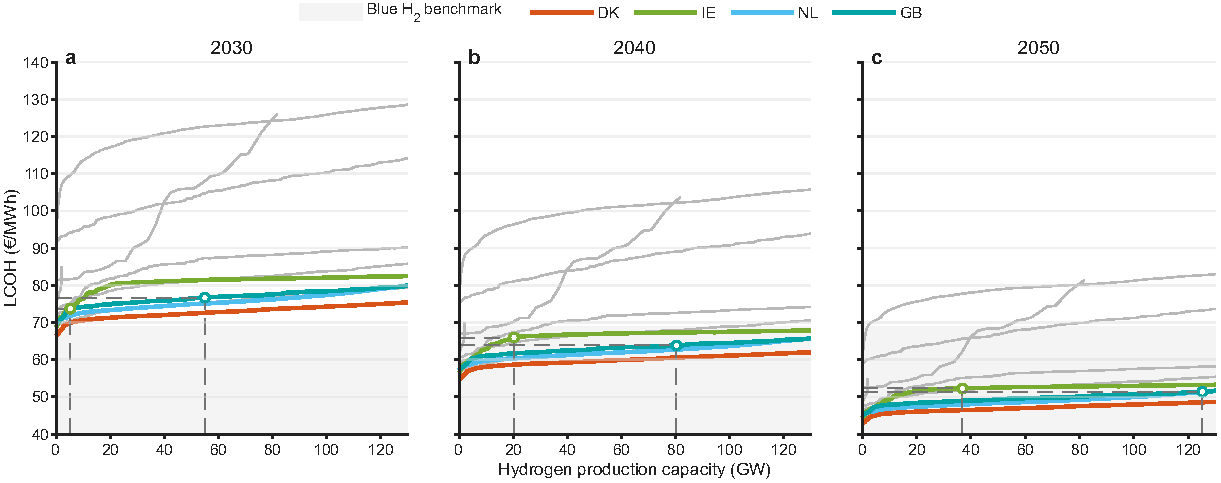
\includegraphics[width = 0.99\columnwidth]{figs/fig_LCOH_curves_manu.pdf}
    \caption{\textbf{Offshore green hydrogen cost-supply curves by country and year.}
    \textbf{a--c}, National cost-supply curves for 2030, 2040 and 2050, respectively. Solid lines denote countries. Markers on Ireland's and the UK's curves indicate their offshore wind capacity targets. Grey shading shows the projected blue-hydrogen cost range.}
    \label{fig LCOH curve}
\end{figure}

% \begin{table*}[]
% \footnotesize
% \caption{Cost-competitiveness of offshore green hydrogen among major countries and with blue hydrogen}
% \label{tab lcoh rank}
% \begin{threeparttable}
% \begin{tabular}{p{1cm}p{2.5cm}p{1cm}p{2.5cm}p{1cm}p{2.5cm}}
% \hline
% 2030 & Average LCOH (€/MWh) & Rank & Marginal LCOH (€/MWh) & Rank & Low-price hydrogen (GW) \\ \hline
% BE   & 74.01                & 4    & 75.21                 & 3    & 0.00                    \\
% DK   & 70.14                & 1    & 71.72                 & 1    & 1.50                    \\
% FR   & 75.76                & 6    & 77.60                 & 6    & 0.00                    \\
% DE   & 73.47                & 2    & 75.12                 & 2    & 0.00                    \\
% IE   & 73.96                & 3    & 76.10                 & 5    & 0.00                    \\
% NL   & 74.36                & 5    & 75.63                 & 4    & 0.00                    \\
% NO   & 87.09                & 9    & 87.09                 & 9    & 0.00                    \\
% PT   & 94.26                & 11   & 94.26                 & 11   & 0.00                    \\
% ES   & 93.32                & 10   & 93.87                 & 10   & 0.00                    \\
% SE   & 76.62                & 8    & 78.48                 & 7    & 0.00                    \\
% GB   & 76.37                & 7    & 79.02                 & 8    & 2.65                    \\ \hline
% 2040 & Average LCOH (€/MWh) & Rank & Marginal LCOH (€/MWh) & Rank & Low-price hydrogen (GW) \\ \hline
% BE   & 61.27                & 3    & 62.57                 & 3    & 14.76                   \\
% DK   & 57.91                & 1    & 59.14                 & 1    & \textgreater{}100       \\
% FR   & 62.45                & 5    & 63.97                 & 5    & 79.58                   \\
% DE   & 60.90                & 2    & 62.44                 & 2    & \textgreater{}100       \\
% IE   & 64.30                & 7    & 67.40                 & 8    & 28.50                   \\
% NL   & 62.05                & 4    & 63.24                 & 4    & \textgreater{}100       \\
% NO   & 73.12                & 9    & 74.21                 & 9    & 0.00                    \\
% PT   & 81.75                & 11   & 85.95                 & 11   & 0.00                    \\
% ES   & 78.14                & 10   & 80.00                 & 10   & 0.00                    \\
% SE   & 64.90                & 8    & 66.71                 & 7    & 62.43                   \\
% GB   & 63.66                & 6    & 65.79                 & 6    & \textgreater{}100       \\ \hline
% 2050 & Average LCOH (€/MWh) & Rank & Marginal LCOH (€/MWh) & Rank & Low-price hydrogen (GW) \\ \hline
% BE   & 48.08                & 2    & 49.10                 & 2    & 14.91                   \\
% DK   & 46.71                & 1    & 47.76                 & 1    & \textgreater{}100       \\
% FR   & 49.95                & 5    & 51.52                 & 5    & \textgreater{}100       \\
% DE   & 48.56                & 3    & 50.09                 & 4    & \textgreater{}100       \\
% IE   & 52.02                & 8    & 54.42                 & 8    & \textgreater{}100       \\
% NL   & 48.87                & 4    & 49.94                 & 3    & \textgreater{}100       \\
% NO   & 57.84                & 9    & 59.20                 & 9    & \textgreater{}100       \\
% PT   & 64.14                & 11   & 67.44                 & 11   & 0.75                    \\
% ES   & 62.14                & 10   & 64.33                 & 10   & 52.74                   \\
% SE   & 51.92                & 7    & 53.24                 & 7    & \textgreater{}100       \\
% GB   & 50.73                & 6    & 52.51                 & 6    & \textgreater{}100       \\ \hline
% \end{tabular}
% \begin{tablenotes}
%     \item Rank means the ranks of average/marginal LCOH among 11 countries; Marginal means the LCOH at the offshore capacity of that country in the corresponding year; Average means the LCOH of sum-up average of all offshore wind capacities in the corresponding year; Low-price hydrogen means the capacity of hydrogen production whose production cost is lower than the upper bound of blue hydrogen.
% \end{tablenotes}
% \end{threeparttable}
% \end{table*}

\begin{figure}
    \centering
    
\includegraphics[width = 0.8\columnwidth]{figs/fig_cost_table.pdf}
    \caption{\textbf{Country rankings for offshore green hydrogen cost competitiveness.}
    \textbf{a--c}, Cost-competitiveness metrics for 2030, 2040 and 2050, respectively. Cell numbers report average and marginal LCOH ranks among the 11 countries, and colours show the underlying LCOH values. Marginal LCOH is evaluated at each country's offshore wind capacity target, whereas average LCOH is calculated across the national cost-supply curve. Circles show the hydrogen production capacity with LCOH below the upper bound of the blue-hydrogen benchmark; the smallest and largest circles denote 0 and >100 GW, respectively.}
    \label{fig lcoh rank}
\end{figure}

\subsection{Domestic offshore wind integration and hydrogen export potential}

Because the ambitious offshore wind capacity targets in Ireland and the UK are much higher than their power demands, we analyse the integration potential of domestic energy systems to determine the export potential of green hydrogen. A whole energy system optimisation approach is used to simulate operating conditions hour by hour across a whole year with uncertain offshore wind generation. The power and natural gas systems are deeply interconnected through gas-fired power plants and on/offshore electrolysers, which are optimised simultaneously to expand flexibility for the accommodation of offshore wind fluctuations. Green hydrogen can be blended into the natural gas network at varying ratios, allowing bulk transport and enabling the analysis to cover future scenarios from zero hydrogen to pure hydrogen networks.
Hourly unit commitment is conducted considering all available generations in the All-Ireland power system, including coal, waste, peat, natural gas, oil, onshore wind, solar, hydro, and offshore wind. The analysis also accounts for practical operating codes designed by EirGrid \cite{OperationalPolicy} for future operation scenarios, such as ramping, interconnectors, inertial constraints, must-run units, and SNSP, together with actual hourly power demand curves (see the supporting information for detailed methodologies, including Supplementary Figs. 14--17 and Supplementary Table 5).

The unit commitment results and wind curtail rate in different seasons, years, and with/without exporting options are compared in Fig.\ref{fig unit commitment}. Considering that the UK government has allowed 20\% hydrogen blending at the distribution level in specific areas, it is assumed the gas transmission network is ready for a maximum 20\% blending ratio in 2040. In 2050, pure hydrogen networks are constructed in line with the UK's hydrogen network roadmap \cite{BritainsHydrogenNetworkPlan}.
As we can see from Fig.\ref{fig unit commitment} a to Fig.\ref{fig unit commitment} c, from 2030 to 2050 in summer, with the increase in offshore wind capacity, the average wind curtailment rate without export generally increases from 67.51\% to 71.29\%. The high wind curtailment is mainly caused by the large difference in high available wind generation and low demand.
In the winter, owing to the fewer wind resources, the average wind curtailment rate decreases by 56.25\% from 2030 to 2050. This is because, in this scenario, the increase in hydrogen blending ratio plays a dominant role, which allows the gas system to absorb more wind.

However, we can observe that even after replacing all natural gas with hydrogen and fully exploiting the flexibility of the energy system, a considerable proportion of offshore wind will still be curtailed mainly due to low domestic energy demand. This highlights the necessity of exporting hydrogen to other countries.
The hydrogen export access could significantly promote offshore wind utilization across all years and all seasons of scenarios, if we compare the upper six figures (Fig.\ref{fig unit commitment} a-f) with the lower six figures (Fig.\ref{fig unit commitment} g-l). For example, the average wind curtailment rate in the 2050 summer can be reduced to 11.53\%. The exporting potential for Ireland is huge (average 27 GW in Fig. \ref{fig unit commitment} i, even 1.68 times higher than total domestic energy demand).
The uncertainty of offshore wind requires operating reserves to be scheduled ahead of real-time operation. High costs of operating reserves and policies on reserve capacity, inertia, and must-run units prevent energy systems from accommodating a certain portion of marginal offshore wind. However, this marginal value does not grow with the year and offshore capacity, so it is interesting to observe that with export options available, the wind curtailment rate even decreases with the increase of offshore wind capacity, which is opposite to the case without export options.


\begin{figure}
    \centering
    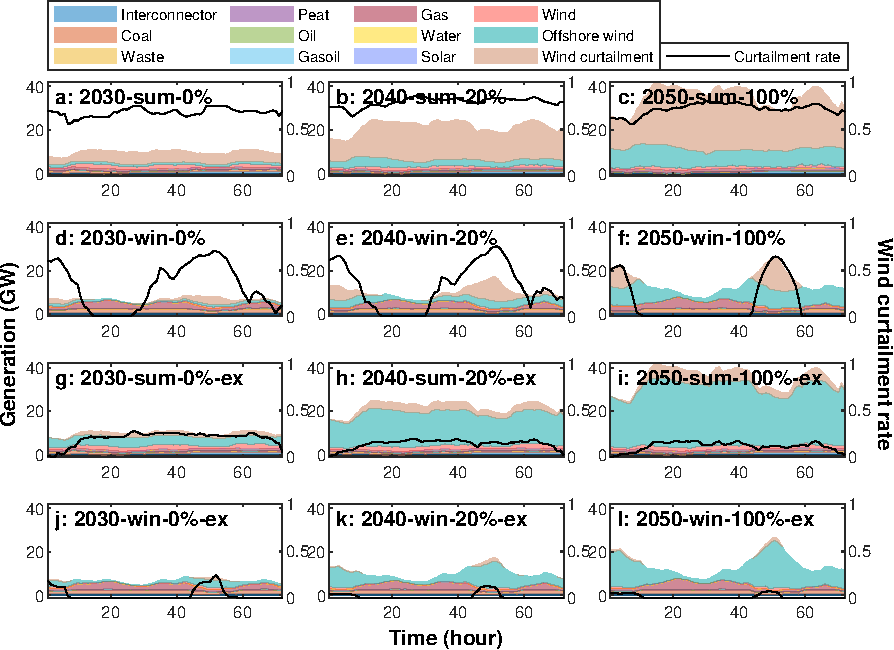
\includegraphics[width = 0.99\columnwidth]{figs/fig_unit_commitment_main.pdf}
    \caption{\textbf{Power system operation results.} Different years, seasons, hydrogen blending ratios, and export conditions, are compared. 2030, 2040, and 2050 indicate the year; sum and win mean a typical summer day (high wind and low demand) and a typical winter day (low wind and high demand), respectively; 0\%, 20\%, and 100\% mean different maximum allowed hydrogen blending potential; ex means export.
   }
    \label{fig unit commitment}
\end{figure}

Using the whole year's results from Ireland, we estimated the offshore wind utilization status for other countries. We assume the offshore wind consumption is proportional to the electricity and gas demand (the domestic-absorption sensitivity is reported in Supplementary Table 7).
The annual offshore wind utilization is decomposed in Fig. \ref{fig wind decomposition}. Among these countries, the UK is leading in offshore wind capacities, and the domestic load is not very high, thus it has the highest exporting potential of 178 TWh in 2030. The Netherlands, Denmark, and Ireland are following after it, with 65, 30, and 16 TWh exporting potential, respectively.
In 2040, although the UK's offshore capacity growth is relatively slower than its energy demand, it and the Netherlands are still the top two exporting countries. On the other hand, because Ireland's offshore capacity has quadrupled to 20 GW while the energy demand increase is much slower, its exporting potential reaches 86 TWh, surpassing Denmark and becoming the third-largest hydrogen exporting country.
In 2050, with access to 100\% hydrogen in natural gas systems, the offshore wind consumption potential from domestic energy systems will increase, especially for countries relying on natural gas generation. Therefore, although the offshore capacities further increase, the exporting potential of the Netherlands even decreases by 13.87\%.
For countries with relatively lower offshore potential and higher domestic energy demands like Germany and France, although their offshore wind capacities are also considerable, there is no green hydrogen left for export.
On the contrary, the hydrogen export potentials from the UK and Ireland continue to increase significantly by 32.59\% and 96.82\% respectively compared with 2040. The UK is leading first place with 232 TWh capacity. Notably, Ireland, with 167 TWh exporting availability, due to its large offshore capacity and low energy demands, exceeds Denmark and the Netherlands to become the second-largest hydrogen exporting country in Europe.

% 能不能也估计一下其他国家电力系统的运行情况，包括切风什么的，然后都画在圆环里。因为是从负荷计算来的，所以不会显得等比例
\begin{figure}
    \centering
    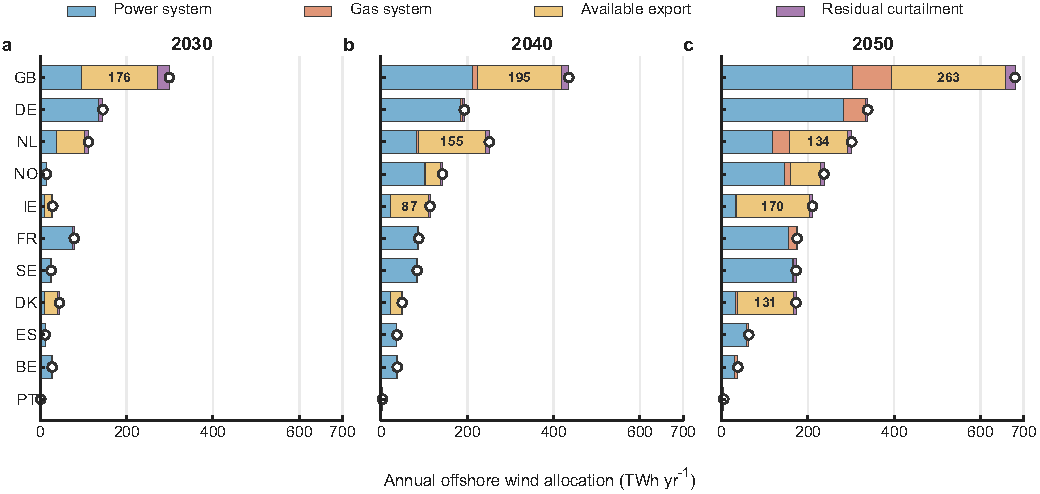
\includegraphics[width = 0.99\columnwidth]{figs/fig_wind_decomposition.pdf}
    \caption{\textbf{Utilisation of offshore wind.}
    \textbf{a}, \textbf{b}, and \textbf{c} decouple the utilisation of wind in 2030, 2040, and 2050, respectively.}
    \label{fig wind decomposition}
\end{figure}

\subsection{Carbon emission mitigation potential in Europe}

\begin{figure}
    \centering
    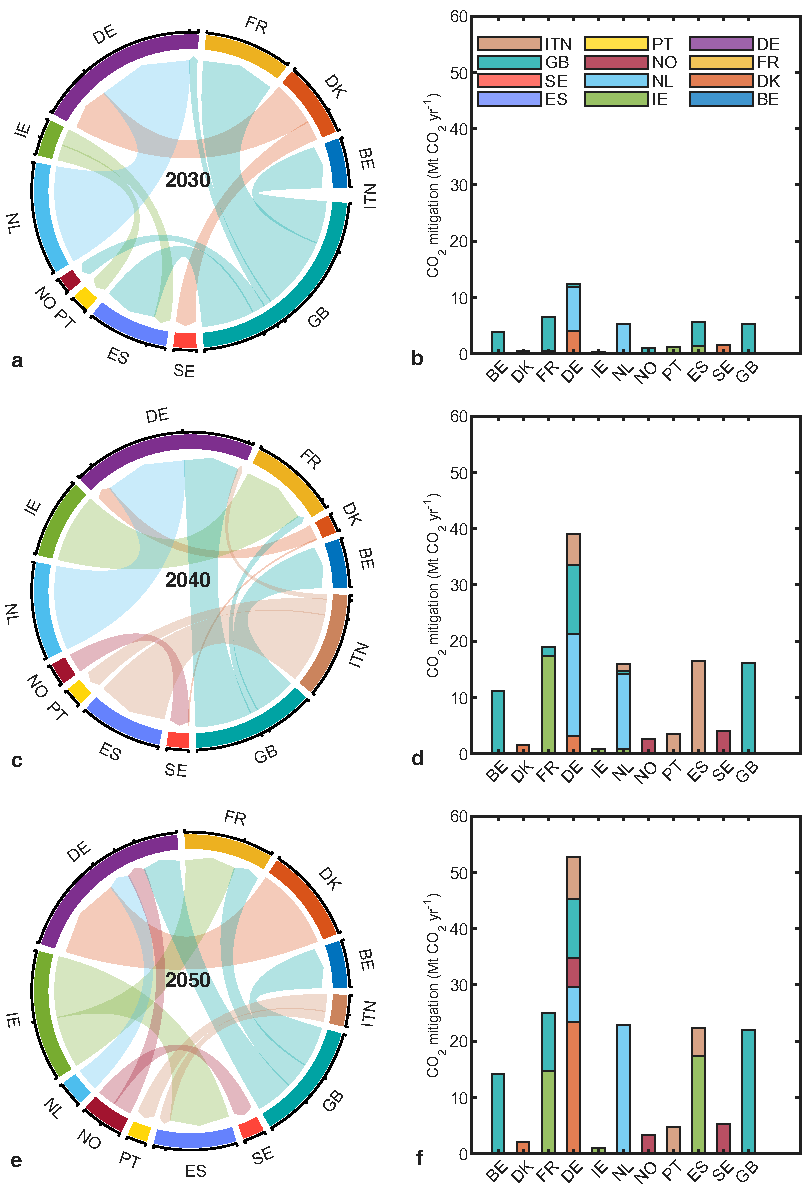
\includegraphics[width = 0.7\columnwidth]{figs/fig_hy_am_flow_sankey.pdf}
    \caption{\textbf{Sankey diagram of hydrogen flows and contributions to decarbonization}
    \textbf{a}, \textbf{c}, and \textbf{e}, are the Sankey diagrams of hydrogen flows among these countries and international hydrogen imports in 2030, 2040, and 2050, respectively. ITN represents international hydrogen import. Please note that only the hydrogen flows between countries are drawn. The hydrogen supplied by and to itself is not indicated in these figures. \textbf{b}, \textbf{d}, and \textbf{f} show the contributions to the decarbonization of each country by international green hydrogen trading. Different bars represent the reduction in carbon dioxide emissions, and different colours indicate different countries' contributions.}
    \label{fig sankey}
\end{figure}
% 多设定一些对比条件，画对比图

% \begin{figure}
%     \centering
%     
\includegraphics[width = 0.99\columnwidth]{figs/fig hy flow manu.pdf}
%     \caption{\textbf{Offshore green hydrogen flows in 2050}
%     The different colours filling the countries indicate the quantity of imported/exported hydrogen. Arrows show the hydrogen flow directions among countries, and the numbers indicate the quality of the hydrogen flow.}
%     \label{fig hy flow}
% \end{figure}

By combining the cost-supply curves and exporting potential analysis in previous sections, here we developed an optimal international green hydrogen trading model to simulate the hydrogen flows among countries in future scenarios. The cost-supply curves are interpolated as piecewise linear functions. Together with shipping costs, they are modelled as objective functions and the optimisation model maximises the decarbonisation with minimal cost. The demand and shipping-cost inputs are shown in Supplementary Figs. 18 and 19. The Sankey diagram of hydrogen flows, reduction of carbon emission, and future hydrogen trading landscape, are shown in Fig. \ref{fig sankey}.

In 2030, the UK will be the major hydrogen exporter, followed by the Netherlands, Denmark, and Ireland. It contributes to 98.29\%, 98.38\%, 26.08\%, and 83.99\% of the hydrogen demands of Belgium, France, Germany, and Spain, respectively.
Germany is the major hydrogen receiver due to its high demand. Besides the UK, 25.72\% and 46.80\% of Germany's hydrogen demand vacancy is fulfilled by Denmark and the Netherlands, owing to the low hydrogen production cost, nearby locations and consequently lower shipping cost.
When it comes to 2040, a major change in the hydrogen trading structure is that the international hydrogen import becomes essential in fulfilling the hydrogen demand, due to the slow offshore capacity growth relative to the hydrogen demand growth. The share of the UK in the hydrogen supply market decreases dramatically. It is no longer able to supply Germany's hydrogen demands after meeting Belgium and France. As a result, Germany will have to import 102 TWh of hydrogen from international markets (such as Eastern Europe and South Africa). The hydrogen demands in Norway, Portugal, and Spain are partially covered by international imports as well. In contrast, we can witness the growth of Ireland's market share at this stage, which supplies 28 and 52 TWh of hydrogen to France and Spain, respectively.
In 2050, as the electrification approaches the end phase and the increase in hydrogen demand slows down, the hydrogen import from the international market will reduce, but will still play an important role in the overall hydrogen supply structure, and will continue its contribution to Germany and Portugal. The reduced share of international hydrogen and the Netherlands is now covered by Ireland.
Though the hydrogen production capacity of Ireland is still lower than the UK, the hydrogen export flow increases to 161 TWh, for the first time exceeding the UK and becoming the largest hydrogen exporter in Europe.

The contributions of hydrogen export and import are also reflected in the reduction of carbon emission, as shown in Fig. \ref{fig sankey} b, d, and f, with accounting values summarised in Supplementary Table 8. In general, the offshore hydrogen production from these 11 countries can contribute to 43.53, 129.32, and 175.16 Mt annual carbon dioxide emission reductions in 2030, 2040, and 2050, respectively, equivalent to 0.74, 2.20 and 2.98 times of Ireland's current carbon emission \cite{COemissions}. In 2030, the UK and the Netherlands will be the main contributors to carbon reduction. Then from 2040 and 2050, similar to the hydrogen supply structure, the importance of Ireland increases gradually. Ireland and the UK, not only account for all carbon mitigation in their own country (1.05 and 21.93 Mt, respectively), but also help the decarbonization of other countries in Europe (33.45 and 27.21 Mt in total).



\subsection{Comparison with a lowest-LCOH allocation}

The integrated trade result can be compared with a simpler allocation based only on offshore production cost. We constructed a lowest-LCOH-only counterfactual that allocates hydrogen demand to the lowest-cost offshore supply first, and compared it with the integrated model that includes domestic absorption limits, shipping costs, national demand and residual external imports. This counterfactual is not intended as a market-design proposal; it is a diagnostic baseline for testing whether the exporter ranking can be inferred from LCOH alone. The modelling-feature comparison is summarised in Supplementary Table 1.

The two approaches give different exporter geographies (Fig. \ref{fig nc lcoh counterfactual}). In the cost-only baseline, the leading net exporters are Denmark in 2030, the Netherlands in 2040 and Denmark again in 2050, with net exports of 44, 147 and 171 TWh yr$^{-1}$, respectively. In the integrated model, the leading net exporter is the UK in all three model years, with 78, 122 and 162 TWh yr$^{-1}$, while Ireland nearly matches the UK in 2050 at 162 TWh yr$^{-1}$. The difference is particularly large in 2050: the cost-only baseline assigns 41 TWh yr$^{-1}$ of net exports to Ireland and a 44 TWh yr$^{-1}$ net import position to the UK, whereas the integrated model increases both countries to approximately 162 TWh yr$^{-1}$ of net exports. The integrated model also reveals residual external import requirements of approximately 116 and 62 TWh yr$^{-1}$ in 2040 and 2050, while the cost-only baseline hides this shortage by construction. The comparison indicates that the policy-relevant exporter ranking is determined by the system balance between cost, domestic absorption, shipping and demand, rather than by LCOH ranking alone.

\begin{figure}[H]
    \centering
    
\includegraphics[width = 0.99\columnwidth]{figs/fig_nc_lcoh_counterfactual.pdf}
    \caption{\textbf{Net-export balances under cost-only and integrated allocation.} \textbf{a} Country net-export balance under a lowest-LCOH-only baseline and the integrated model in 2030, 2040 and 2050. Blue indicates net export and red indicates net import. Black boxes mark the leading net exporter in each model-year combination. \textbf{b} Leading net exporter and corresponding net export under the two model structures. \textbf{c} Residual outside imports identified by the integrated model. The cost-only baseline allocates demand within the modelled European offshore supply by construction and therefore does not expose the residual external import requirement.}
    \label{fig nc lcoh counterfactual}
\end{figure}

\subsection{Sensitivity to external import prices}

The UK/Ireland export result is strong, but not unconditional. It depends on how attractive non-European low-carbon hydrogen or ammonia imports become relative to European offshore supply. This outside option is strategically important because European policy already anticipates substantial renewable hydrogen imports, while the future scale, timing and cost of global low-emission hydrogen trade remain uncertain \cite{EuropeanCommissionHydrogen2026,IEAGlobalHydrogenReview2025,IEAGlobalHydrogenReviewTrade2025}. We therefore replaced the previous high import penalty with a delivered hydrogen-equivalent outside-option price and solved the trade model over 2.0--6.0 EUR kg$^{-1}$ H$_2$-equivalent in 0.1 EUR kg$^{-1}$ increments. This range should be read as a threshold scan rather than a price forecast: its low end is informed by optimistic global trade and cost estimates, while the upper range represents less favourable delivery, infrastructure, finance or policy conditions \cite{IRENAGlobalHydrogenTradeOutlook2022,IRENAGreenHydrogenCostPotential2022}.

The outside-option scan shows a threshold rather than a smooth robustness band (Fig. \ref{fig nc outside option robustness}). Across all three model years, European offshore supply is absent at 2.0 EUR kg$^{-1}$ H$_2$-equivalent and first enters the solution at 2.8 EUR kg$^{-1}$, but it only becomes the majority source near 3.1 EUR kg$^{-1}$ in 2030 and 3.3 EUR kg$^{-1}$ in 2040--2050 (Fig. \ref{fig nc outside option robustness}a). In the 2050 case, offshore supply increases from 98 TWh yr$^{-1}$ at 3.0 EUR kg$^{-1}$ to about 600 TWh yr$^{-1}$ at 3.3 EUR kg$^{-1}$ and 709 TWh yr$^{-1}$ at 3.5 EUR kg$^{-1}$, while outside imports fall from approximately 721 to 226 and 119 TWh yr$^{-1}$. The carbon-mitigation attribution shifts in the same direction, from being dominated by the external option to being dominated by European offshore suppliers (Fig. \ref{fig nc outside option robustness}b). The country-level response shows why this boundary matters for strategic geography: once the price reaches about 3.5 EUR kg$^{-1}$, the UK, Ireland and Denmark re-emerge as large net exporters at approximately 162, 157 and 118 TWh yr$^{-1}$, respectively, while Germany, France and Spain remain large net importers (Fig. \ref{fig nc outside option robustness}c). Higher outside-option prices leave this allocation largely unchanged, so the result should be read as a boundary condition on the integrated conclusion rather than as a graded price forecast.

\begin{figure}[H]
    \centering
    
\includegraphics[width = 0.99\columnwidth]{figs/fig_nc_outside_option_robustness.pdf}
    \caption{\textbf{European offshore supply under external import price sensitivity.} \textbf{a} Supply-regime ribbons across model years and delivered outside-option prices resolved in 0.1 EUR kg$^{-1}$ increments. Orange indicates external low-carbon imports and blue indicates European offshore supply; right-hand labels give total modelled demand in each year. \textbf{b} 2050 carbon-mitigation attribution shifts from the external outside option to European offshore suppliers as the outside-option price crosses the boundary. \textbf{c} Country net-export shifts across the 3.0--3.5 EUR kg$^{-1}$ H$_2$-equivalent boundary in 2050. Orange and blue points show the 3.0 and 3.5 EUR kg$^{-1}$ solutions, respectively. The scan identifies a delivered-price boundary rather than assigning probabilities to future import prices.}
    \label{fig nc outside option robustness}
\end{figure}

\section{Discussion}

Cross-border offshore hydrogen trade can convert Atlantic offshore wind surplus into European carbon-mitigation value, but the resulting exporter geography differs from a production-cost ranking. Denmark remains the strongest cost-competitiveness benchmark across the cost-supply curves, but Ireland and the UK become strategically important only after domestic absorption, national demand, shipping and residual external imports are considered together. In the integrated 2050 case, the UK and Ireland become the two largest net exporters with approximately 162 TWh yr$^{-1}$ each, followed by Denmark with approximately 118 TWh yr$^{-1}$.

The comparison with a lowest-cost-only allocation clarifies the planning implication. That allocation identifies Denmark or the Netherlands as the leading exporters and hides residual import dependence. The integrated model instead identifies a west-to-east trade structure with persistent external import needs in 2040 and 2050. The result is therefore not that high-resource island countries automatically dominate offshore hydrogen trade. Rather, their strategic role emerges when large offshore build-out coincides with limited domestic absorption, nearby continental demand and a delivered external import option that is not ultra-low cost.

These findings also clarify how Ireland should be interpreted in future hydrogen planning. Ireland has no decisive LCOH advantage and does not have the largest offshore hydrogen production capacity. Its strategic value arises from the combination of sufficient cost competitiveness, large exportable surplus and European demand centres that remain undersupplied by their domestic offshore resources. This conclusion supports considering multiple export corridors and carrier options rather than evaluating Irish exports only through a single pipeline route. It also implies that national offshore hydrogen strategies should be assessed within a regional trade and demand balance, not only through domestic cost-supply estimates.

The contribution of this study is therefore methodological as well as quantitative. By linking geospatial offshore hydrogen cost-supply curves, hourly domestic power-gas absorption, hydrogen/ammonia shipping and an explicit external import option, the model exposes a ranking reversal that single-module assessments cannot capture. The lowest-LCOH baseline points to Denmark or the Netherlands as leading exporters, but the integrated model identifies the UK as the leading exporter in all three model years and Ireland as an almost equal exporter by 2050. This integrated European-scale treatment makes the UK/Ireland result visible and provides a direct test of why production-cost maps alone are insufficient for export strategy.

The conclusions are bounded by three design choices. The analysis uses currently published offshore wind goals and therefore assumes that planned infrastructure is delivered on schedule. Domestic absorption outside Ireland is estimated by scaling the Ireland hourly whole-system result with national electricity and gas demand, so the export-potential estimates should be read as a European screening result rather than a replacement for country-specific unit-commitment studies. We stress-test this bridge in the Supplementary Information by resolving the integrated trade model after multiplying domestic absorption by 0.75 and 1.25. This changes European offshore supply, residual imports and the exact UK/Ireland ordering, but it does not restore the LCOH-only exporter geography: Ireland remains a leading net exporter and the ranking reversal relative to the cost-only baseline is preserved. The outside-option analysis is also a threshold scan, not a forecast of future global hydrogen prices. These bounds identify where country-level planning and future market evidence would most improve the analysis.

The results indicate that residual external imports remain necessary in the integrated 2040 and 2050 cases, at approximately 116 and 62 TWh yr$^{-1}$, respectively. More ambitious offshore hydrogen production goals could reduce this dependence, especially in countries with lower marginal costs and remaining offshore capacity potential, such as Denmark and the Netherlands. Infrastructure policy also matters. Offshore wind turbines, electrolysers, subsea cables, ports and hydrogen shipping vessels must be coordinated with stable regulation, faster consenting and dedicated export corridors. Otherwise, European hydrogen demand can grow faster than domestic offshore supply.

These findings give a practical test for future hydrogen strategies. Countries should not be ranked only by LCOH or offshore resource quality. They should be evaluated by their position in the wider system: domestic absorption, exportable surplus, carrier choice, shipping access, demand geography and competing external imports. In that system view, Ireland and the UK become strategic exporters because large offshore surplus, shipping access and nearby demand align, not because they sit at the top of a cost ranking.



\section{Methods}\label{sec11}

\subsection{Model workflow and scope}

We built the workflow to quantify cross-border offshore hydrogen trade and its carbon-mitigation attribution under domestic-system and import-competition constraints. The workflow links geospatial supply mapping, hourly domestic system operation, European trade optimisation and carbon-displacement accounting. Offshore wind, bathymetry, port-distance, grid-connection and exclusion-area data define country-level cost-supply curves for offshore hydrogen in 2030, 2040 and 2050. A coordinated domestic operation model estimates the share of offshore production that can be absorbed before an export outlet is needed. The remaining export potential enters a European trade model in which hydrogen can move as hydrogen or ammonia, and demand can also be met by an external import option. The optimised delivery matrix is then translated into supplier-attributed carbon-mitigation values. The Methods give the system boundary and assumptions needed to interpret the results; algebraic formulations and parameter tables are reported in the Supplementary Information.

The model covers Belgium, Denmark, France, Germany, Ireland, the Netherlands, Norway, Portugal, Spain, Sweden and the UK. Each model year is solved independently for 2030, 2040 and 2050. Energy flows are optimised as average power quantities and converted to TWh yr$^{-1}$ for reporting. Carbon-mitigation outputs are reported in Mt CO$_2$ yr$^{-1}$.

\subsection{Techno-economic mapping of offshore hydrogen supply}

The supply module estimates where offshore hydrogen can be produced and at what cost within the EEZs of the selected coastal European countries \cite{Marineregions}. Aquaculture sites, Special Areas of Conservation and military areas are excluded from the developable offshore hydrogen production area using EMODnet boundaries \cite{EMODnet}. Within the remaining offshore grid cells, hourly wind velocity, temperature and air-pressure data are taken from the ERA5 reanalysis at 1 h temporal resolution and $0.5^\circ \times 0.5^\circ$ spatial resolution, equivalent to approximately 45 km by 56 km in southern Europe \cite{ERA5}.

Hourly wind generation is calculated from the power curve of an NREL reference 15 MW wind turbine \cite{musial2019oregon}. The turbine power curve is defined at 1 m s$^{-1}$ wind-speed increments, with linear interpolation for intermediate wind speeds. Turbine layouts are chosen by balancing power density against wake losses rather than imposing a uniform turbine spacing. Single-turbine wakes are represented with the Jensen-Gaussian model \cite{tao2019optimal}. For overlapping wakes from multiple upstream turbines, we use a recursive-tree method that reduces simulation time by 79\% with less than 1\% accuracy loss in benchmark tests \cite{Figshare}, avoiding the computational burden of enumerating many wake combinations across long historical weather series \cite{paul2019multi, tao2020joint}. Further methodological details and parameter values are provided in the Supplementary Information.

LCOH is calculated with a bottom-up representation of development expenditure, capital expenditure, operational expenditure and decommissioning expenditure. European techno-economic parameters, including environmental survey, wind-turbine and cable costs, are taken from Offshore Renewable Energy Catapult \cite{OffshoreWindandHydrogen}; the detailed cost breakdown is provided in the Supplementary Information.

The site-specific cost calculation depends on water depth, capacity factor, distance to the nearest port, distance to the nearest connection point and turbine spacing. Bathymetry data are obtained from EMODnet and converted to $0.001^\circ \times 0.001^\circ$ grid cells, equivalent to approximately 0.11 km by 0.06 km near the UK \cite{bathymetry_2022}. Water depth determines whether monopile, jacket or floating turbine structures are technically applicable and affects foundation material requirements. Depths below 30 m are treated as suitable for monopiles, depths of 30--60 m for jacket foundations, and depths above 60 m for floating foundations. Port distance affects installation and maintenance costs, while distance to connection points affects export-cable CAPEX. Turbine spacing is selected so that wake interference from adjacent turbines remains below 5\%, which also determines the array-cable length used in the cost calculation.

Offshore hydrogen production is represented as an integrated wind-electrolysis platform with water pumping and desalination, alkaline electrolysers, hydrogen compressors, standby batteries and auxiliary offshore infrastructure. Alkaline electrolysis is used because it is currently a mature and durable electrolyser option for large-scale deployment; techno-economic characteristics are summarised in Supplementary Table 4. Capital-cost and electrical-efficiency projections are taken from Offshore Renewable Energy Catapult and the UK's National Hydrogen Strategy, with alkaline-electrolyser efficiency increasing from 0.79 in 2030 to 0.82 in 2050 \cite{HydrogenAnalyticalAnnex}. Annual OPEX includes maintenance, stack replacement and labour costs as a percentage of initial capital investment.

Because variable offshore wind output can differ from the electrolyser operating point, the platform includes electrical and hydrogen storage. Water pumping, desalination and compression loads are sized with hydrogen production, so their power consumption scales with hydrogen production capacity. Algebraic sizing equations are used to maximise utilisation and determine the electrolyser and accessory capacities (Supplementary Information, Section 3.3). Future operating parameters and cost projections are taken from Offshore Renewable Energy Catapult \cite{OffshoreWindandHydrogen}. LCOH is then calculated for the combined wind farm, electrolysis system and offshore auxiliaries.

Cost-supply curves are generated by ranking grid-cell production segments by LCOH and accumulating the available hydrogen quantity. The potential installed offshore wind capacity for each grid cell is calculated from turbine rated power and the maximum number of turbines that can be placed in the cell under the wake-interference constraint. Vessel density, obtained from EMODnet at 1 km resolution, reduces available power density linearly up to a maximum 50\% reduction \cite{RouteDensityMap, guo2023grid}. Future LCOH reductions are represented through high, median and low technology-learning scenarios based on expert elicitation \cite{wiser2021expert}. Under the median scenario, relative to 2020, fixed-bottom offshore wind costs are reduced by 21\%, 35\% and 49\% in 2030, 2040 and 2050, respectively; floating offshore wind costs are reduced by 2\%, 17\% and 40\%.


\subsection{Domestic absorption of offshore wind and hydrogen}

The domestic model quantifies a binding system limit: how much offshore energy can be used inside the All-Island power and gas systems before exports create additional value. Offshore electricity is connected to the power system by marine cables, while offshore hydrogen can enter the gas system through blending or, in the 2050 case, a pure-hydrogen network assumption. The scenario hydrogen fraction in the gas network is set to 0\% in 2030, 20\% in 2040 and 100\% in 2050. These cases represent a transition from no material blending, through an intermediate blending limit, to a dedicated hydrogen-network case. The 20\% case reflects current blending demonstrations and policy discussion \cite{EuropeanHydrogenBackbone, HyDeploy, HyBlend, HydrogenblendinginGB}, while the 2050 case is aligned with hydrogen-network planning \cite{BritainsHydrogen}.

The coordinated model determines hourly operation over a representative year while minimising operating cost and maximising offshore-resource integration subject to power-system and gas-system constraints. We use paired export and no-export cases to separate offshore wind that can be absorbed domestically from offshore wind that requires an external hydrogen or ammonia outlet. The resulting quantities define domestic offshore wind use, hydrogen production, curtailment and exportable surplus.

The power side is represented by a nodal unit-commitment model that balances electricity demand and uncertain renewable generation. The objective includes thermal-unit fuel costs and start-up costs, with operational constraints for ramping, minimum online and offline times, minimum output levels, must-run units and reserves. The model also represents the operational policy roadmap for the All-Island system, including inertia, minimum numbers of conventional units and System Non-Synchronous Penetration limits \cite{OperationalPolicyRoadmap}. Network congestion is represented with DC power flow. Seasonal dynamic line ratings are included for summer and winter cases, and planned interconnection expansion, including the 700 MW Celtic Interconnector with France, is represented \cite{CelticInterconnector}.

The gas side captures the operational effect of hydrogen injection from offshore electrolysis. Hydrogen blending changes gas composition and therefore changes the heat value, specific gravity and safety characteristics of the gas mixture. We define an admissible gas-quality region using the Gas Safety (Management) (Amendment) Regulations 2023, including relative density, Wobbe index and Weaver flame-speed factor limits \cite{TheGasSafety2023}. Gas flow and pressure are represented with the Weymouth equation. Because variable gas composition introduces additional non-convexity, the gas-flow problem is solved using the previously developed reformulation framework based on McCormick envelopes, second-order cone reformulation and sequential convex programming \cite{wang2023optimal}. Gas streams with different compositions are mixed at pipeline junctions; the resulting bilinear terms are handled with the same solution framework. Mathematical details are provided in Supplementary Information, Section 4.

The coordinated operation model is parameterised with detailed All-Island generation, demand and network data. Generator capacities, piecewise heat-rate curves and operating parameters are obtained from the Single Electricity Market model used in EirGrid publications \cite{SEMPLEXOS}. Commodity costs and heat values are represented for non-gas fossil-fuel units. For gas-fired units, fuel use is linked to the gas-system calculation so that heat value changes with hydrogen fraction. Onshore wind and solar generation are calculated from ERA5 wind speed and solar-radiation data; photovoltaic output is calculated using the Beckman model. Hydropower generation is taken from historical operation data \cite{SystemandRenewableDataReports}.

Future gas demand is based on Gas Networks Ireland's Gas Forecast Statement and reflects coal-plant retirements, the 80\% renewable-generation ambition in Ireland's Climate Action Plan, restrictions on new gas boiler connections, GDP-linked residential, industrial and commercial demand changes, and compressed natural gas station development \cite{GasForecastStatement2022}. Daily electricity peak demands to 2032 are taken from EirGrid's Ten-Year Generation Capacity Statement for winter, summer and spring-autumn cases \cite{GenerationCapacity}. Missing values between 2033 and 2050 are filled using an autoregressive integrated moving average model. Fifteen-minute electricity and gas demand profiles are taken from EirGrid's smart-grid dashboard and the Gas Networks Ireland data dashboard \cite{SmartGridDashboard, GasconsumptionbyMarketSector}. High-voltage power lines above 110 kV and high-pressure gas pipelines above 16 bar are represented using network topology, location and parameter data from EirGrid and Gas Networks Ireland \cite{AllIslandTenYear, NetworkDevelopmentPlan}. Gas-pipeline friction factors and diameters follow an Ireland case study \cite{ekhtiari2022green}; power-line capacities are assumed to grow at the same annual rate as demand.

\subsection{European hydrogen and ammonia trade optimisation}
The trade model asks where residual offshore supply is used once domestic absorption has been accounted for. It combines the country-level cost-supply curves and export-potential estimates with hydrogen and ammonia demand, shipping costs, domestic self-supply and an external import option in 2030, 2040 and 2050. Countries with published offshore wind targets, including Ireland \cite{FutureFrameworkforOffshore} and the UK \cite{Offshorewindnet}, use those targets as maximum offshore capacities. For countries without complete year-specific targets, we use tentative goals from the European Union's non-binding agreement on offshore wind deployment \cite{Offshorerenewableenergy}. Hydrogen and ammonia demands are taken from the European Hydrogen Backbone demand projection \cite{Analysingfuturedemand}.

The optimisation minimises total production, shipping and external-import costs subject to national offshore supply capacities, domestic export limits, country-level demand, shipping-route capacities and material balances. National production, bilateral carrier flows, route-level vessel deployment and external imports are chosen simultaneously. Hydrogen and ammonia production costs are represented through piecewise-linear interpolations of the cost-supply curves. Shipping costs include annualised vessel investment costs and operating fuel costs, with route distances derived from port-to-port shipping paths \cite{EMODnet}. Because the supply curves and vessel-count decisions introduce discrete choices, the model is formulated as a mixed-integer linear programming problem and solved in MATLAB using Gurobi. The complete formulation is given in Supplementary Information, Section 5.

The international import node acts as an outside option rather than as an additional European supplier. It is retained in the base integrated model so that demand can still be met when European offshore supply is insufficient. In the outside-option sensitivity, the same node is assigned a delivered hydrogen-equivalent price and the model is solved repeatedly over 2.0--6.0 EUR kg$^{-1}$ H$_2$-equivalent in 0.1 EUR kg$^{-1}$ increments, corresponding approximately to 60--180 EUR MWh$^{-1}$. Hydrogen and ammonia imports are assigned the same hydrogen-equivalent delivered price so that the scan isolates the threshold at which European offshore supply becomes competitive with non-European low-carbon imports.

We use carbon mitigation as an attribution metric rather than a full lifecycle assessment. Optimised hydrogen and ammonia deliveries are converted to avoided CO$_2$ using the carrier-specific conversion factors defined in the Supplementary Information and assigned to a supplier-destination contribution matrix. Positive bilateral route variables assign the avoided CO$_2$ to the exporting country and importing country; negative route variables reverse the direction before assignment. Domestic self-supply is assigned to the matrix diagonal, and the external import node is reported separately from the 11 European offshore supplier countries. The total carbon mitigation reported in the main text is the sum of the full matrix, while the European offshore supplier contribution excludes the external import row.

To separate the integrated result from a cost-only interpretation, we construct a lowest-LCOH counterfactual in which total European hydrogen and ammonia demand is allocated to offshore supply segments in ascending LCOH order. This baseline uses planned offshore capacity and capacity factors to limit country supply, but deliberately excludes domestic absorption limits, shipping costs, demand geography and the competitive external-import price. It is therefore used only as a diagnostic baseline for testing whether exporter rankings can be inferred from production cost alone.

\backmatter

\section*{Acknowledgments}

This work was supported by the Newcastle University Academic Track (NUAcT) Fellowship.

\section*{Author contributions}

S.W. conceived the study, developed the modelling framework and MATLAB code, performed the analysis, prepared the figures and wrote the original manuscript. M.M.B. contributed to the energy-system interpretation, policy context and manuscript review and editing. Both authors reviewed and approved the final manuscript.

\section*{Competing interests}

The authors declare no competing interests.

\section*{Data availability}

The public data sources used in this study are cited in the References and described in the Methods and Supplementary Information. Derived source-data tables generated by the analysis, including the headline-number audit table used to trace manuscript values and a source-data coverage inventory, are available in the project repository under \verb|results/tables/|. Final figure files are provided under \verb|manuscript/figs/|. Large public raw climate, bathymetry and geospatial inputs and large intermediate MATLAB checkpoint files are not redistributed through the GitHub repository because of file-size constraints; the raw inputs are available from the cited public data providers and the checkpoints can be regenerated from the provided code.

\section*{Code availability}

MATLAB code used in this study is available on GitHub at \url{https://github.com/ShengWang-EE/HyExport}.


% supplementary information
\begin{appendices}

% \section{Supplementary information}
\bmhead{Supplementary information}






\end{appendices}

%%===========================================================================================%%
%% If you are submitting to one of the Nature Portfolio journals, using the eJP submission   %%
%% system, please include the references within the manuscript file itself. You may do this  %%
%% by copying the reference list from your .bbl file, paste it into the main manuscript .tex %%
%% file, and delete the associated \verb+\bibliography+ commands.                            %%
%%===========================================================================================%%

\bibliography{sn-bibliography}% common bib file
%% if required, the content of .bbl file can be included here once bbl is generated
%%\input sn-article.bbl

% \section*{Supplementary information}

\end{document}
